%Fiquemos com Deus e Nossa Senhora!
%Sao Jose de Cupertino rogai por nos!!
% ### Uses XeLaTeX ### %
% ### Needs beamer-master ### %
\documentclass[aspectratio=169]{beamer} %. Aspect Ratio 16:9

\usetheme{AI2} % beamerthemeSprace.sty
\usepackage[portuguese]{babel}
\usepackage[utf8]{inputenc}
\usepackage[T1]{fontenc}
\usepackage{ragged2e,gensymb}

\DeclareMathOperator*{\argmin}{arg\,min}
\DeclareMathOperator*{\argmax}{arg\,max}
\DeclareMathOperator{\sign}{sgn}

% DATA FOR FOOTER
\date{2021}
\title{- Máquinas de Vetores de Suporte}
\author{João Paulo Papa}
\institute{Advanced Institute for Artificial Intelligence (AI2)}

\begin{document}
% ####################################
% FIRST SLIDE 						:: \SliTit{This is the Title of the Talk}{A. B. Name}{Sprace}
% SUB-TITLE SLIDE 					:: \SliSubTit{<title>}{<explanation}
% SUB-SUB-TITLE SLIDE				:: \SliSubSubTit{<title>}{<explanation}
% SLIDE WITH TITLE 					:: \SliT{Title}{Content}
% SLIDE NO TITLE 						:: \Sli{Content} 
% SLIDE DOUBLE COLUMN WITH TITLE 	:: \SliDT{Title}{First Column}{Second Column}
% SLIDE DOUBLE COLUMN NO TITLE 		:: \SliD{First Column}{Second Column}
% SLIDE ADVANCED WITH TITLE 			:: \SliAdvT{Title}{Content}
% SLIDE ADVANCED NO TITLE 			:: \SliAdv{Content}
% SLIDE ADVANCED DOUBLE WITH TITLE 	:: \SliAdvDT{Title}{First Column}{Second Column}
% SLIDE ADVANCED DOUBLE NO TITLE 	:: \SliAdvD{First Column}{Second Column}
% SLIDE BLACK						:: \Black{ <Content> }
% SLIDE WHITE						:: \White{ <Content> }
% ITEMIZATION 						:: \begin{itemize}  \iOn{First} \iTw {Second} \iTh{Third} \end{itemize}
% COMMENT TEXT				 		:: \note{<comment>}
% SECTION 							:: \secx{Section} | \secxx{Sub-Section}
% BOLD SPRACE COLOR				:: \bfs{<text>}
% TABLE OF CONTENT					:: \tocitem{<title>}{<content>}
% LEFT ALIGN EQUATION				:: \begin{flalign*}  & <equation> &   \end{flalign*}
% CENTER ALIGN EQUATION	S			:: \begin{gather*} <equations>  \end{gather*}
% SLASH								:: \slashed{<>}
% BAR								:: \barr{<letter>} instead of \bar{<letter>}
% THEREFORE						:: use \portanto (larger and bold}
% 2 or 3 MATH SYMBOLS				:: \overset{<up>}{<down>} &  \underset{<below>}{\overset{<above>}{<middle>}}  
% INSERT TEXT IN FORMULA			:: \ins{<text>}
% EXERCISE							:: \exe{<exercise #>}{<exercise text>}
% SUGGESTED READING BOX			:: \sug{<references>}
% CITATION							:: \cittex{<citation>}
% CITATION DOUBLE COLUMN 			:: \cittexD{<citation>}
% TEXT POSITION						:: \texpos{<Xcm>}{<Ycm>}{<text>} origin = center of slide : x right | y down
% REFERENCE AT BOTTOM  S/D SLIDE		:: \refbotS{<reference>} \refbotD{<reference>}
% HIDDEN SLIDE						:: \hid
% COLOR BOX 						:: \blu{blue} + \red{rec} + \yel{yellow} + \gre{green} + \bege{beige}
% FRAME 							:: \fra{sprace} \frab{blue} \frar{red} + \fray{yellow} + \frag{green}		
% FIGURE 							:: \img{X}{Y}{<scale>}{Figure.png} 
% FIGURE							:: \includegraphics[scale=<scale>]{Figures/.png}
% FIGURE DOUBLE SLIDE NO TITLE		::  \img{-4}{0.5}{<scale>}{Figure.png} % Image 1st half
%									::  \img{4}{0.5}{<scale>}{Figure.png} % Image 2nd half
% FIGURE DOUBLE SLIDE WITH TITLE		::  \img{-4}{0}{<scale>}{Figure.png} % Image 1st half
%									::  \img{4}{0}{<scale>}{Figure.png} % Image 2nd half
% INCLUDING SWF (Flash)				:: \usepackage{media9} and \includemedia >> USE ACROBAT <<
%%%%%%%%%%%%%%%%%%%%%%%%%%%%%%%%%%%%%%%%%%%%%%%%%%
% ###############################################################################
% FIRST SLIDE
\SliTit{{\LARGE Máquinas de Vetores de Suporte}}{Advanced Institute for Artificial Intelligence -- AI2}{https://advancedinstitute.ai}
%%%%%%%%%%%%%%%%%%%%%%%%%%%%%%%%%%%%%%%%%%%%%%%%%%
% ###############################################################################
% SLIDE SUB-TITLE
%\SliSubTit{Sub-Title}{Description}{}
%%%%%%%%%%%%%%%%%%%%%%%%%%%%%%%%%%%%%%%%%%%%%%%%%%
% ###############################################################################
%\SliSubSubTit{Sub-Sub-Title}{Description}
 %%%%%%%%%%%%%%%%%%%%%%%%%%%%%%%%%%%%%%%%%%%%%%%%%%


\SliT{Introdução}{

\justifying As Máquinas de Vetores de Suporte, do inglês \emph{Support Vector Machines} (SVM) são baseadas em conceitos da Teoria do Aprendizado Estatístico (TAE), desenvolvida por Vapnik e colegas. Basicamente, a ideia seria estudar garantias teóricas sobre condições necessárias para o processo de aprendizado.

\justifying Como dito anteriormente, temos duas principais limitações durante um processo de aprendizagem:

\begin{itemize}
	\item supertreinamento (\emph{overfitting}): baixa capacidade de generalização no conjunto de teste.
	\item subtreinamento (\emph{underfitting}): baixa capacidade de aprendizado no conjunto de treinamento.
\end{itemize}
}

\Sli{
\justifying Qual seria a situação ideal? Um \textbf{compromisso} entre as duas situações, ou seja, uma relação custo-benefício entre supertreinamento e subtreinamento. 

\justifying \underline{Definição do problema}: dado um espaço de funções ${\cal F}$, como escolher uma função $\hat{f}\in{\cal F}$ de tal forma que o erro no treinamento seja baixo e a capacidade de generalização seja alta? A TAE nos fornece condições para atingir este objetivo sem assumir uma formulação específica para a distribuição dos dados (abordagem não paramétrica).

\justifying \underline{Objetivo}: Encontrar o melhor classificador $f^\ast\in{\cal F}$ para um conjunto de treinamento fixo com tamanho $m$ de tal forma que se aproxime, ao máximo, do classificador de menor risco, ou seja, $f_{bayes}$.
}

\Sli{
\justifying Quando o aprendizado é \textbf{consistente}, ou seja, quando $f^\ast$ consegue aprender dos dados? Primeiramente, precisamos definir o espaço de funções ${\cal F}$ que o nosso classificador fará parte. Vamos analisar a figura abaixo.

\begin{minipage}{0.43\textwidth}
\begin{center}
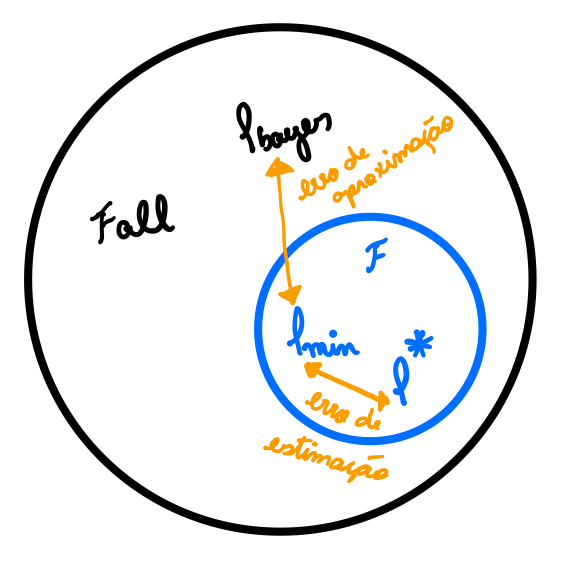
\includegraphics[scale=0.21]{./figs/SVM_Fig1.png}
\end{center}
\end{minipage}%%% to prevent a space
\begin{minipage}{0.49\textwidth}
\begin{itemize}
	\item ${\cal F}_{all}$: espaço de todas as funções possíveis
	\item ${\cal F}$: espaço das funções que o classificador pode aprender
	\item $f_{bayes}$: classificador de mínimo risco possível
	\item $f_{min}$: classificador de mínimo risco em ${\cal F}$
\end{itemize}
\null
\par\xdef\tpd{\the\prevdepth}
\end{minipage}
}

\Sli{
\justify Podemos, então, associar um \textbf{risco} $R$ à cada classificador. Desta forma, $R(f^\ast)$ corresponde ao risco associado ao classificador $f^\ast$.

\justify Temos que um classificador é dito ser \textbf{consistente} se, e somente se, o seu risco é minimizado quando $m\rightarrow\infty$, ou seja, quando o conjunto de treinamento aumenta. Em outras palavras, a consistência nos diz se estamos conseguindo aprender ou não.

\justify O grande problema é que, quando ${\cal F}\rightarrow{\cal F}_{all}$, o nosso aprendizado não é consistente, pois o espaço de funções possíveis aumenta muito. Assim, devemos restringir o tamanho de ${\cal F}$. No entanto, o nosso dilema é: \textbf{ao restringirmos ${\cal F}$, o nosso erro de aproximação fica grande; ao ampliarmos ${\cal F}$, o nosso erro de estimação aumenta.}
}

\Sli{
\justify A pergunta principal é: \textbf{como escolher ${\cal F}\subset{\cal F}_{all}$ e $f^\ast\in{\cal F}$?} A TAE nos ajuda a responder à essa questão propondo as SVMs, que é uma classe de (funções) classificadores ótimas no que diz respeito ao \textbf{compromisso} entre os erros de aproximação e estimação.

\justify \underline{Objetivo}: encontrar um hiperplano que maximize a \textbf{margem} de segurança e cometa poucos \textbf{erros marginais}, isto é, minimize o risco. O que são erros marginais?

\begin{center}
\begin{tabular}{cc}
	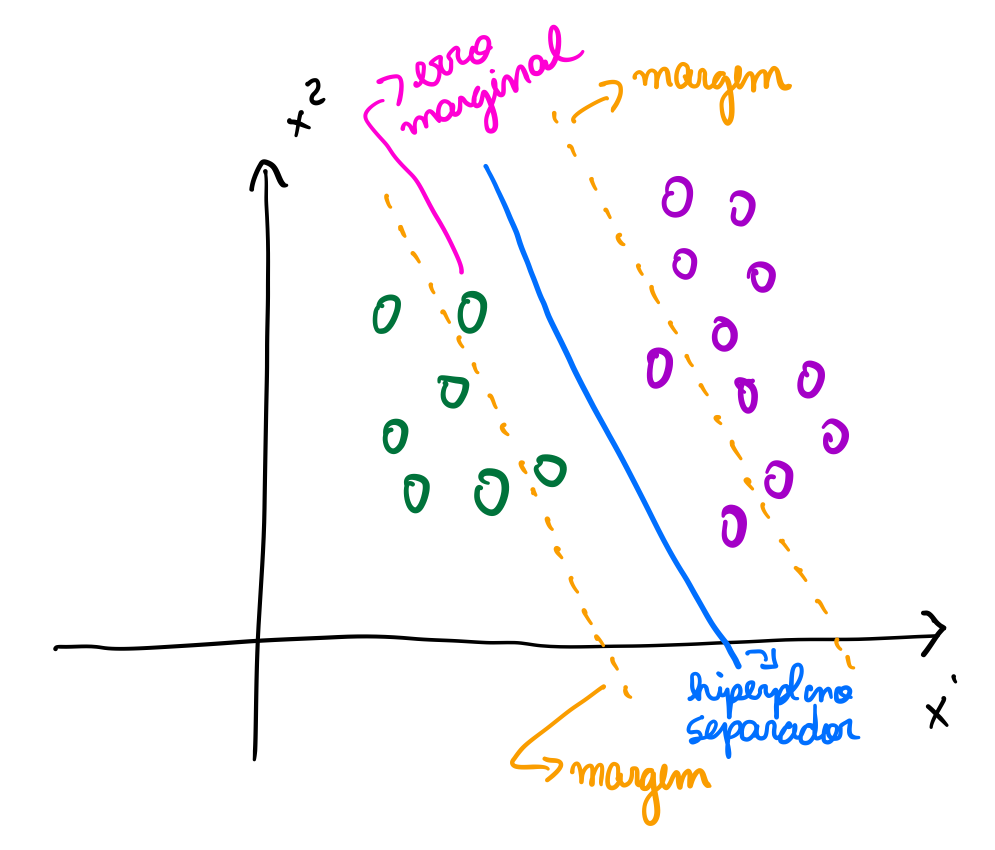
\includegraphics[scale=0.15]{./figs/SVM_Fig2.png} &\hspace{2cm}
	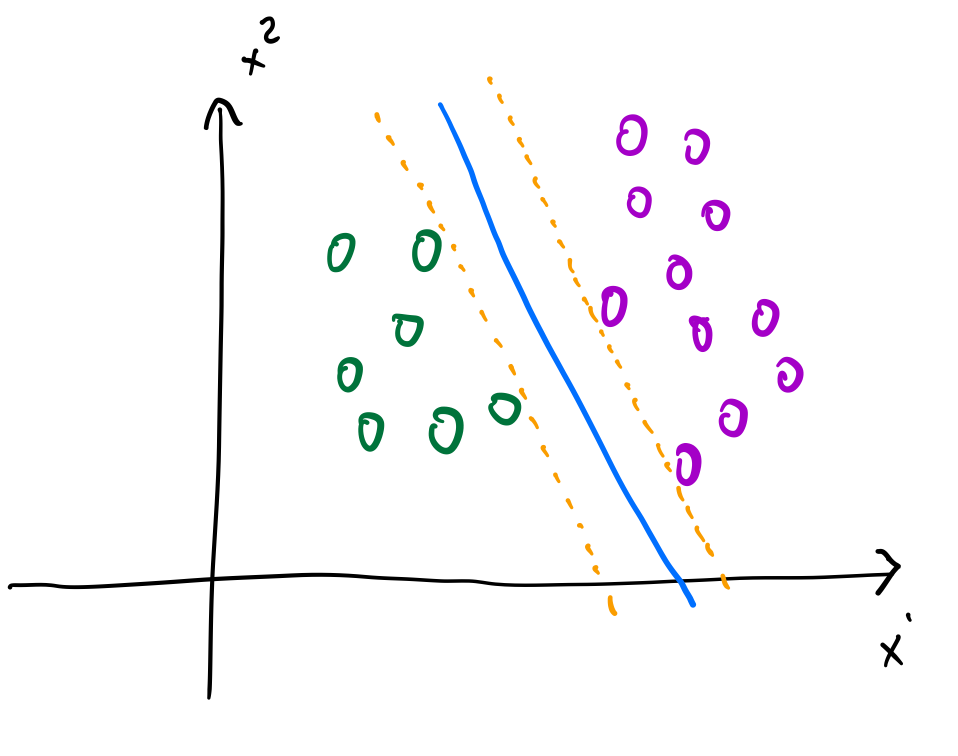
\includegraphics[scale=0.15]{./figs/SVM_Fig3.png}
\end{tabular}
\end{center}
}

\Sli{
\justify Fazemos uma analogia com o algoritmo do Perceptron no sentido que ambos utilizam uma função de decisão linear, ou seja, um hiperplano. A diferença é que o hiperplano do Perceptron não possui as \textbf{propriedades ótimas} que o hiperplano encontrado pelo SVM possui.

\begin{center}
\begin{tabular}{cc}
	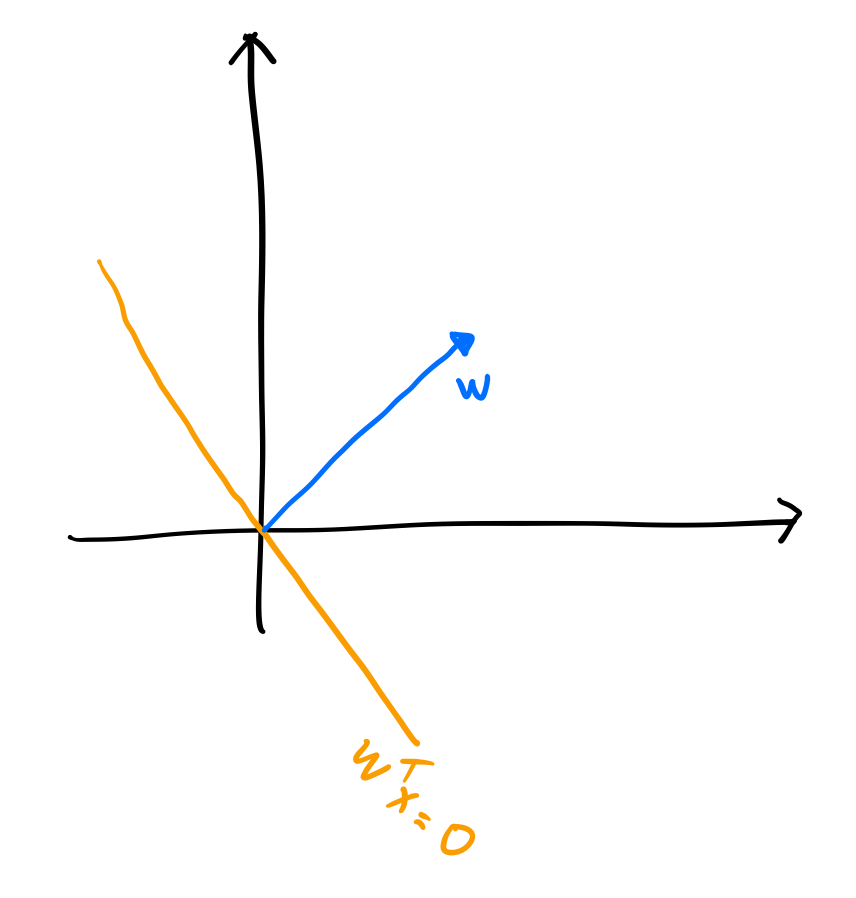
\includegraphics[scale=0.19]{./figs/SVM_Fig4.png} &\hspace{1cm}
	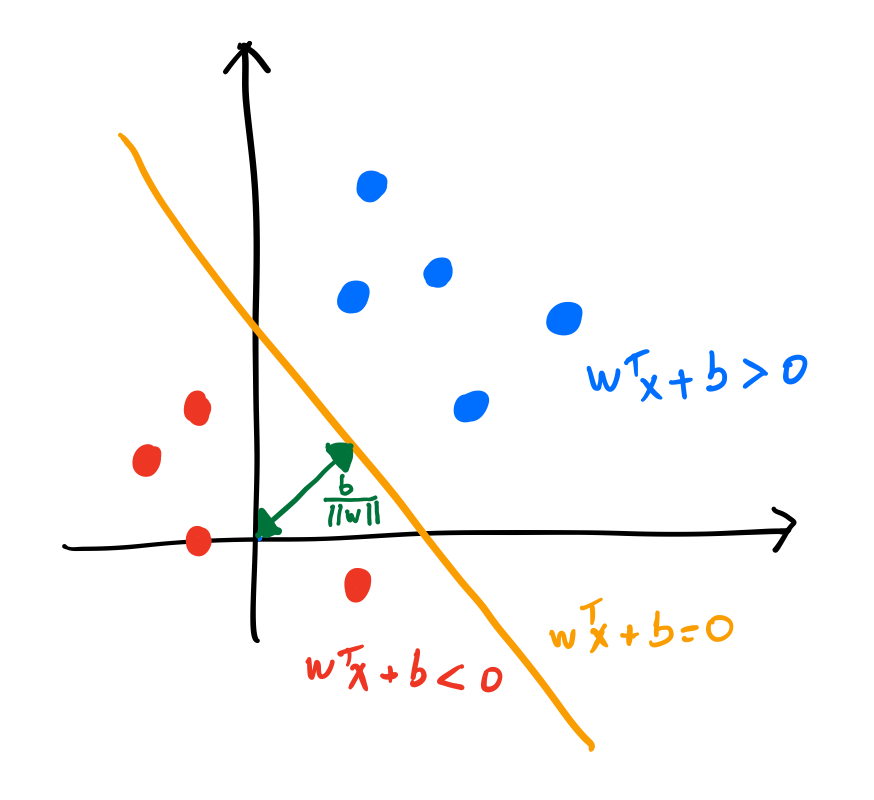
\includegraphics[scale=0.19]{./figs/SVM_Fig5.png}
\end{tabular}
\end{center}\vspace{-1cm}
}

\Sli{
\justify Definimos, também, como \textbf{hiplerplano canônico} $H$ aquele cujas amostras mais próximas satisfaçam $|\boldsymbol{w}^T\boldsymbol{x}+\theta|=1$. Como ilustrado abaixo, temos que os hiperplanos $H_1$ e $H_2$ definem, então, as margens com relação ao hiperplano canônico. 

\begin{center}
	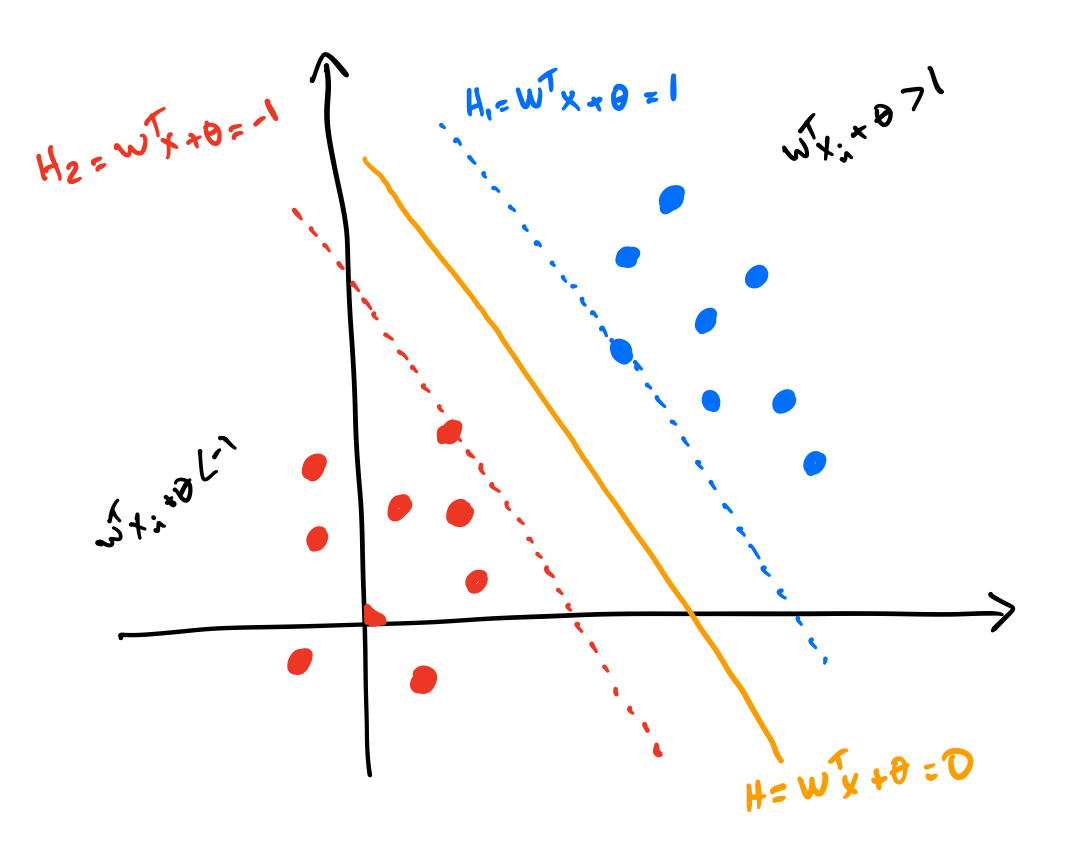
\includegraphics[scale=0.19]{./figs/SVM_Fig6.png}
\end{center}
}

\Sli{
\justify \underline{Definição do problema:} dado um conjunto de treinamento rotulado, isto é, classificação supervisionada, ${\cal X}^1=\{(\boldsymbol{x}_1,y_1),(\boldsymbol{x}_2,y_2),\ldots,(\boldsymbol{x}_m,y_m)\}$, as amostras mais próximas do hiperplano canônico $H$ devem satisfazer as seguintes condições:

\begin{itemize}
	\item $H_1:\boldsymbol{w}^T\boldsymbol{x}_i+\theta=1\implies \boldsymbol{w}^T\boldsymbol{x}_i+(\theta-1)=0$
	\item $H_2:\boldsymbol{w}^T\boldsymbol{x}_i+\theta=-1\implies \boldsymbol{w}^T\boldsymbol{x}_i+(\theta+1)=0$
\end{itemize}

\justify Em termos de classificação, temos que:

\begin{equation}\nonumber
	\boldsymbol{w}^T\boldsymbol{x}_i+\theta \leq -1\text{ se $y_i = -1$}
\end{equation}
e
\begin{equation}\nonumber
	\boldsymbol{w}^T\boldsymbol{x}_i+\theta \geq 1\text{ se $y_i = 1$}.
\end{equation}
}

\Sli{
Podemos unificar as equações anteriores da seguinte forma:

\begin{equation}
	y_i(\boldsymbol{w}^T\boldsymbol{x}_i+\theta)-1\geq 0,
\end{equation}
que é conhecida pela \textbf{restrição do problema}. 

\justify Note que teremos $m$ restrições, ou seja, uma para cada amostra do conjunto de treinamento, o que é bastante custoso para o classificador. Esse é um dos motivos que torna o SVM uma técnica bastante cara computacionalmente, sendo um dos seus principais pontos negativos.
}

\Sli{
Como podemos calcular a distância $d(H_1,h_2)$ entre os hiperplanos?

\begin{minipage}{0.43\textwidth}
\begin{center}
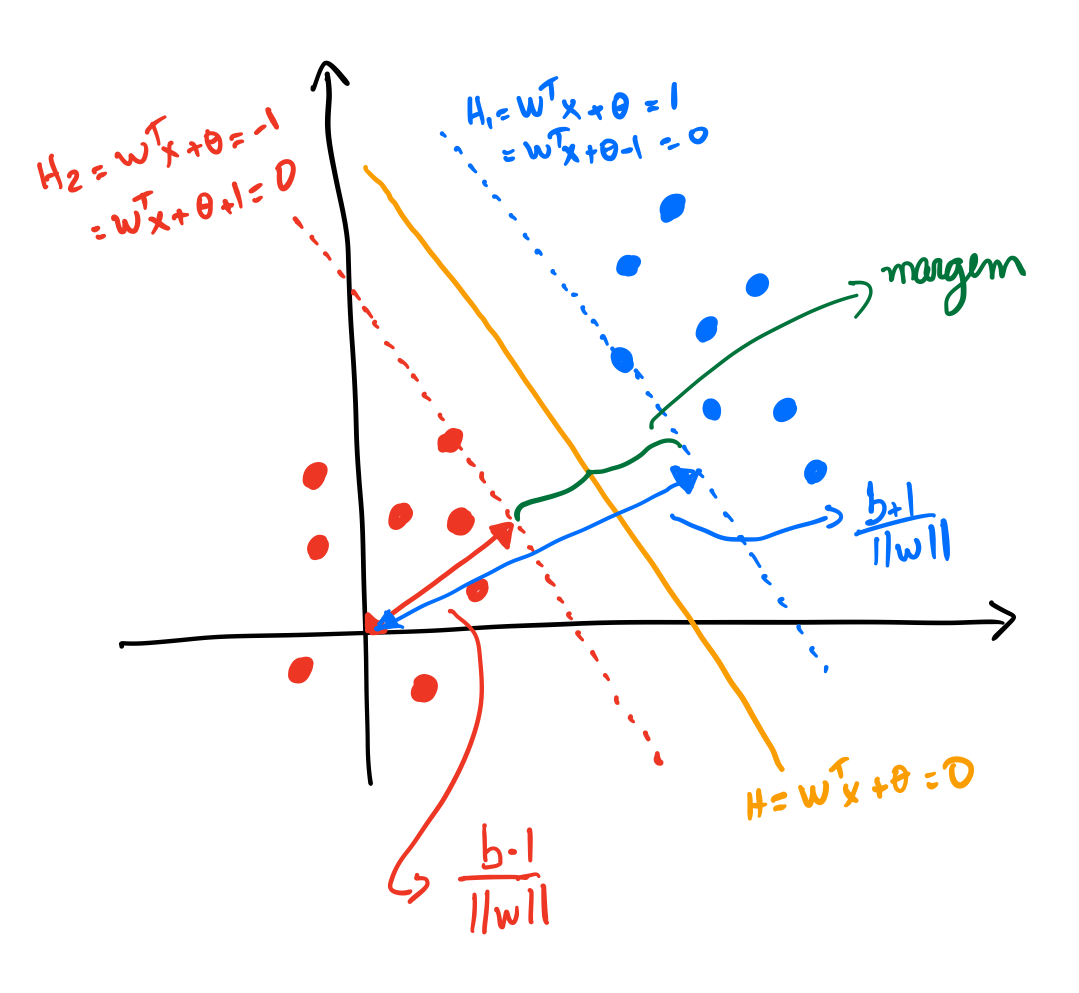
\includegraphics[scale=0.17]{./figs/SVM_Fig7.png}
\end{center}
\end{minipage}%%% to prevent a space
\begin{minipage}{0.49\textwidth}
\begin{align}\nonumber
	d(H_1,h_2) &= \frac{\theta+1}{\norm{\boldsymbol{w}}}-\frac{\theta-1}{\norm{\boldsymbol{w}}}\\
	&= \frac{(\theta+1)-(\theta-1)}{\norm{\boldsymbol{w}}}\\\nonumber
	&= \frac{\theta+1-\theta+1}{\norm{\boldsymbol{w}}}\\\nonumber
	&= \frac{2}{\norm{\boldsymbol{w}}}	\nonumber
\end{align}
\null
\par\xdef\tpd{\the\prevdepth}
\end{minipage}
}

\Sli{
Desta forma, para \textbf{maximizar} a margem de separação, devemos \textbf{minimizar} $\norm{\boldsymbol{w}}$. Assim sendo, temos o seguinte problema de otimização:

\begin{equation}
	\boldsymbol{w}^\ast,\theta^\ast = \argmin_{\boldsymbol{w},\theta}\frac{1}{2}\norm{\boldsymbol{w}}^2,
\end{equation}
sujeito às seguintes restrições:

\begin{equation}\nonumber
	y_i(\boldsymbol{w}^T\boldsymbol{x}_i+\theta)-1\geq 0,\ \ \ \forall i=1,2,\ldots,m.
\end{equation}
As restrições acima garantem que não existem dados de treinamento entre os hiperplanos de separação.
}

\Sli{
\justify Quando temos um problema de otimização sujeito à restrições de desigualdade, utilizamos duas principais ferramentas matemáticas: condições \textbf{KKT} (Karush–Kuhn–Tucker) e os chamados \textbf{Multiplicadores de Lagrange}.

\justify O primeiro passo para a resolução da Equação 3 é criar a função Lagrangiana, a qual vai incorporar as restrições na própria função objetivo:

\begin{equation}
	L(\boldsymbol{w}, \theta, \boldsymbol{\alpha}) = \frac{1}{2}\norm{\boldsymbol{w}}^2-\sum_{i=1}^m\alpha_i[y_i(\boldsymbol{w}^T\boldsymbol{x}_i+\theta)-1],
\end{equation}
também conhecida como forma \textbf{primal} do problema de otimização, em que $\boldsymbol{\alpha}\in\mathbb{R}^m$ denota os multiplicadores de Lagrange.
}

\Sli{
O nosso problema agora passar a ser a otimizar a função Lagrangiana dada pela Equação 4, o que implica em encontrar os valores de $\boldsymbol{\alpha}$, $\boldsymbol{w}$ e $b$ para os quais o gradiente da função é nulo, ou seja:

\begin{equation}
	\nabla L(\boldsymbol{w}, \theta, \boldsymbol{\alpha}) = 0.
\end{equation}
Isto implica que as derivadas parciais em relação aos parâmetros do hiperplano que desejamos encontrar devem ser nulas, ou seja:

\begin{equation}
\frac{\partial L(\boldsymbol{w}, \theta, \boldsymbol{\alpha})}{\partial \theta} = 0
\end{equation}
e
\begin{equation}
\frac{\partial L(\boldsymbol{w}, \theta, \boldsymbol{\alpha})}{\partial \boldsymbol{w}} = 0.	
\end{equation}
}

\Sli{
A derivada parcial com relação ao bias, ou seja, parâmetro $\theta$ é dada como segue:
\vspace{0.35cm}
\begin{align}\nonumber
\frac{\partial L(\boldsymbol{w}, \theta, \boldsymbol{\alpha})}{\partial \theta} &= \frac{1}{2}\norm{\boldsymbol{w}}^2-\sum_{i=1}^m\alpha_i[y_i(\boldsymbol{w}^T\boldsymbol{x}_i+\theta)-1]= 0\\\nonumber
&= \frac{1}{2}\norm{\boldsymbol{w}}^2-\sum_{i=1}^m[\alpha_iy_i(\boldsymbol{w}^T\boldsymbol{x}_i+\theta)-\alpha_i] = 0\\
&= \frac{1}{2}\norm{\boldsymbol{w}}^2-\sum_{i=1}^m\alpha_iy_i(\boldsymbol{w}^T\boldsymbol{x}_i+\theta)+\sum_{i=1}^m\alpha_i = 0\\\nonumber
&= \cancelto{0}{\frac{1}{2}\norm{\boldsymbol{w}}^2}-\sum_{i=1}^m[\cancelto{0}{\alpha_iy_i\boldsymbol{w}^T\boldsymbol{x}_i}+\alpha_iy_i\theta]+\cancelto{0}{\sum_{i=1}^m\alpha_i} = 0\\
&= \sum_{i=1}^m\alpha_iy_i = 0.\nonumber
\end{align}
}

\Sli{
Já a derivada parcial com relação ao vetor $\boldsymbol{w}$ é dada por:
\begin{align}\nonumber
	\frac{\partial L(\boldsymbol{w}, \theta, \boldsymbol{\alpha})}{\partial \boldsymbol{w}} &= \frac{1}{2}\norm{\boldsymbol{w}}^2-\sum_{i=1}^m\alpha_i[y_i(\boldsymbol{w}^T\boldsymbol{x}_i+\theta)-1]= 0\\\nonumber
	&= \boldsymbol{w}-\sum_{i=1}^m[\alpha_iy_i(\boldsymbol{w}^T\boldsymbol{x}_i+\theta)-\alpha_i] = 0\\
	&= \boldsymbol{w}-\sum_{i=1}^m\alpha_iy_i(\boldsymbol{w}^T\boldsymbol{x}_i+\theta)+\sum_{i=1}^m\alpha_i = 0\\\nonumber
	&= \boldsymbol{w}-\sum_{i=1}^m[\alpha_iy_i\boldsymbol{w}^T\boldsymbol{x}_i+\cancelto{0}{\alpha_iy_i\theta}]+\cancelto{0}{\sum_{i=1}^m\alpha_i} = 0\\
	&= \boldsymbol{w}-\sum_{i=1}^m\alpha_iy_i\boldsymbol{x}_i\implies \boldsymbol{w}=\sum_{i=1}^m\alpha_iy_i\boldsymbol{x}_i.\nonumber
\end{align}
}

\Sli{
Substituindo-se as Equações 8 e 9 na forma primal do problema (Equação 4), encontramos a sua forma \textbf{dual}. Relembrando a forma primal, temos que ela é composta por dois termos:

\begin{equation}\nonumber
L(\boldsymbol{w}, \theta, \boldsymbol{\alpha}) = \overbrace{\frac{1}{2}\norm{\boldsymbol{w}}^2}^{\text{Termo 1}}\underbrace{-\sum_{i=1}^m\alpha_i[y_i(\boldsymbol{w}^T\boldsymbol{x}_i+\theta)-1]}_{\text{Termo 2}}.
\end{equation}
Desenvolvendo o primeiro termo e utilizando a Equação 9, temos que:
\begin{align}\nonumber
	\frac{1}{2}\norm{\boldsymbol{w}}^2 &= \frac{1}{2}\boldsymbol{w}^T\boldsymbol{w} = \frac{1}{2}\left(\sum_{i=1}^m\alpha_iy_i\boldsymbol{x}_i\right)^T\left(\sum_{i=1}^m\alpha_iy_i\boldsymbol{x}_i\right)\\
	&= \frac{1}{2}\sum_{i=1}^m\sum_{j=1}^m\alpha_i\alpha_jy_iy_j(\boldsymbol{x}_i^T\boldsymbol{x}_j).
\end{align}
}

\Sli{
Desenvolvendo o segundo termo, temos que:

\begin{align}\nonumber
	-\sum_{i=1}^m\alpha_i[y_i(\boldsymbol{w}^T\boldsymbol{x}_i+\theta)-1] &= -\sum_{i=1}^m\alpha_i[y_i\boldsymbol{w}^T\boldsymbol{x}_i+y_i\theta-1]\\
	&= -\sum_{i=1}^m[\alpha_iy_i\boldsymbol{w}^T\boldsymbol{x}_i+\alpha_iy_i\theta-\alpha_i] \\\nonumber
	&= -\sum_{i=1}^m\alpha_iy_i\boldsymbol{w}^T\boldsymbol{x}_i-\sum_{i=1}^m\alpha_iy_i\theta+\sum_{i=1}^m\alpha_i\\\nonumber
	&= -\sum_{i=1}^m\alpha_iy_i\boldsymbol{w}^T\boldsymbol{x}_i-\theta\sum_{i=1}^m\alpha_iy_i+\sum_{i=1}^m\alpha_i.\\\nonumber
\end{align}
}

\Sli{
Podemos, ainda, desenvolver a Equação 11 um pouco mais. 

\begin{align}\nonumber
	-\sum_{i=1}^m\alpha_iy_i\boldsymbol{w}^T\boldsymbol{x}_i-\theta\cancelto{0\  \text{(Equação 8)}}{\sum_{i=1}^m\alpha_iy_i}+\sum_{i=1}^m\alpha_i &= -\sum_{i=1}^m\alpha_iy_i\boldsymbol{w}^T\boldsymbol{x}_i+\sum_{i=1}^m\alpha_i\\
	&= -\sum_{i=1}^m\alpha_iy_i\underbrace{\left(\sum_{j=1}^m\alpha_jy_jx_j\right)^T\boldsymbol{x}_i}_{\text{Equação 9}}+\sum_{i=1}^m\alpha_i\\\nonumber
	&= -\sum_{i=1}^m\sum_{j=1}^m\alpha_i\alpha_jy_iy_j\boldsymbol{x}_i^T\boldsymbol{x}_j+\sum_{i=1}^m\alpha_i.
\end{align}
}

\Sli{
Substituindo-se, então, as Equações 10 (primeiro termo) e 12 (segundo termo) na Equação 4, temos que:

\begin{align}\nonumber
	L(\boldsymbol{\alpha}) &= \frac{1}{2}\sum_{i=1}^m\sum_{j=1}^m\alpha_i\alpha_jy_iy_j\boldsymbol{x}_i^T\boldsymbol{x}_j-\sum_{i=1}^m\sum_{j=1}^m\alpha_i\alpha_jy_iy_j\boldsymbol{x}_i^T\boldsymbol{x}_j+\sum_{i=1}^m\alpha_i\\
	&= -\frac{1}{2}\sum_{i=1}^m\sum_{j=1}^m\alpha_i\alpha_jy_iy_j\boldsymbol{x}_i^T\boldsymbol{x}_j+\sum_{i=1}^m\alpha_i.
\end{align}
Note que, agora, nossa função objetivo depende apenas dos multiplicadores de Lagrange $\boldsymbol{\alpha}$. Lembre-se que, na Equação 4, nossa função dependia de $\boldsymbol{\alpha}$, $\boldsymbol{w}$ e $b$.
}

\Sli{
\justify Como o problema \textbf{primal} era de \textbf{minimização}, agora o problema \textbf{dual} torna-se uma \textbf{maximização} (teoria de otimização matemática). Assim sendo, nosso problema de otimização consiste em resolver a seguinte formulação:
\vspace{0.17cm}
\begin{align}\nonumber
	\boldsymbol{\alpha}^\ast &= \argmax_{\boldsymbol{\alpha}}\{L(\boldsymbol{\alpha})\}\\
	&= \argmax_{\boldsymbol{\alpha}}\left\{-\frac{1}{2}\sum_{i=1}^m\sum_{j=1}^m\alpha_i\alpha_jy_iy_j\boldsymbol{x}_i^T\boldsymbol{x}_j+\sum_{i=1}^m\alpha_i\right\}, 
\end{align}
sujeito às seguintes restrições:

\begin{equation}\nonumber
	\alpha_i \geq 0,\ \ \forall i=1,2,\ldots,m
\end{equation}
e
\begin{equation}\nonumber
\sum_{i=1}^m\alpha_iy_i = 0.	
\end{equation}
}

\Sli{
\justify Qual a vantagem de termos um problema em sua forma dual? Temos apenas uma variável de interesse, ou seja, $\boldsymbol{\alpha}$. Assim, para resolvermos a Equação 14, precisamos empregar algum método de otimização quadrática (somatório duplo). É por esse motivo que o processo de treinamento do classificador SVM é \textbf{bastante custoso computacionalmente}.

\justify Desta forma, obtendo-se $\boldsymbol{\alpha}^\ast$ por algum método de otimização matemática, basta utilizamos ele na Equação 9 para obtemos $\boldsymbol{w}$. Já para calcularmos o $\theta$, precisamos utilizar as condições de KKT, as quais são condições \textbf{necessárias} para que a solução do problema dado pela Equação 14 seja ótima. Essas condições são dadas pelas seguintes restrições:

\begin{equation}
	\alpha_i^\ast(y_i[(\boldsymbol{w}^\ast)^T\boldsymbol{x}_i+\theta]-1) = 0,\ \forall i=1,2,\ldots,m.
\end{equation}
}

\Sli{
\justify Note que $y_i(\boldsymbol{w}^T\boldsymbol{x}_i+\theta)-1 = 0$ ocorre apenas para as amostras que se encontram \textbf{sobre} os hiperplanos $H_1$ e $H_2$. Assim, $\alpha_i$ pode ser \textbf{não nulo} apenas sobre os elementos $\boldsymbol{x}_i$ que se encontram nesses hiperplanos. Para as demais amostras $\boldsymbol{x}_j$, isto é, aquelas estão estão definidas além das margens, temos que $\alpha_j = 0$ para a condição ser satisfeita.

\justify Para esses elementos cujos multiplicadores de Lagrange são não nulos damos o nome de \textbf{vetores de suporte}. Eles correspondem às amostras \textbf{mais informativas} do conjunto de treinamento, pois estão mais próximas do hiperplano separador. Assim sendo, apenas essas amostras são utilizadas no cálculo de $H$, conforme apresenta a Equação 9.
}

\Sli{
Temos, então, que $\theta^\ast$ pode ser calculado como segue:

\begin{equation}
	\theta^\ast = \frac{1}{|{\cal S}|}\sum_{\boldsymbol{x}_i\in{\cal S}}\left\{\frac{1}{y_i}-(\boldsymbol{w}^\ast)^T\boldsymbol{x}_i\right\},
\end{equation}
em que ${\cal S}\subseteq {\cal X}^1$ denota o conjunto dos vetores de suporte. Podemos, ainda, escrever a equação acima substituindo $\boldsymbol{w}^\ast$ pela Equação 9, isto é, em função dos multiplicadores de Lagrange:

\begin{equation}
	\theta^\ast = \frac{1}{|{\cal S}|}\sum_{\boldsymbol{x}_i\in{\cal S}}\left\{\frac{1}{y_i}-\sum_{\boldsymbol{x}_j\in{\cal S}}\alpha_j^\ast y_j\boldsymbol{x}_j^T\boldsymbol{x}_i\right\}.
\end{equation}
}

\Sli{
A função de decisão (classificação) do SVM apenas retorna o sinal da amostra que está sendo avaliada, ou seja:

\begin{equation}
	h_{\boldsymbol{w}^\ast}(x) = \sign\{(\boldsymbol{w}^\ast)^T\boldsymbol{x}+\theta^\ast\} = \sign\left\{\underbrace{\sum_{\boldsymbol{x}_i\in{\cal S}}y_i\alpha^\ast_i\boldsymbol{x}_i^T}_{\boldsymbol{w}^\ast}\boldsymbol{x}+\theta^\ast\right\}.
\end{equation}
\justify Neste caso, caso $h_{\boldsymbol{w}^\ast}(x)<0$ (sinal negativo), então a amostra é classificada como sendo da classe $-1$; ou da classe $1$ caso contrário. Note que $\boldsymbol{w}^\ast$ controla a \textbf{inclinação} do hiperplano ótimo, $\theta^\ast$ define a sua \textbf{posição} em relação às \textbf{margens}.
}

\SliT{SVMs com Margens Suaves}{
\justify O objetivo dessa variante é lidar com o problema de sobreposição entre as classes permitindo com que algumas amostras possam violar a restrição e situar-se \textbf{entre} as margens.

\justify Lembrando que as restrições originais eram dadas por $y_i(\boldsymbol{w}^T\boldsymbol{x}_i+\theta)\geq 1$, $\forall i=1,2\ldots,m$. Agora, nossas novas restrições são dadas por:

\begin{equation}
	y_i(\boldsymbol{w}^T\boldsymbol{x}_i+\theta)\geq 1-\epsilon_i,
\end{equation}
em que $\epsilon_i\geq 0$ representam as variáveis de folga que possuem o papel de "suavizar"\ as margens.
}

\Sli{
Agora, nossa função objetivo é dada por:

\begin{equation}
	\boldsymbol{w}^\ast,\theta^\ast,\boldsymbol{\epsilon}^\ast = \argmin\left\{\frac{1}{2}\norm{w}^2+C\left(\sum_{i=1}^m\epsilon_i\right)\right\},
\end{equation}
sujeito a $y_i(\boldsymbol{w}^T\boldsymbol{x}_i+\theta)\geq 1-\epsilon_i$, em que $\epsilon_i\in[0,1]$ indica que os dados estão entre as margens. Note que o parâmetro $C$ controla a relação custo-benefício entre SVMs de margens rígidas e margens suaves.
}

\Sli{
\justify A ideia, então, é permitir que amostras estejam posicionadas entre as margens, conforme ilustrado abaixo.

\begin{center}
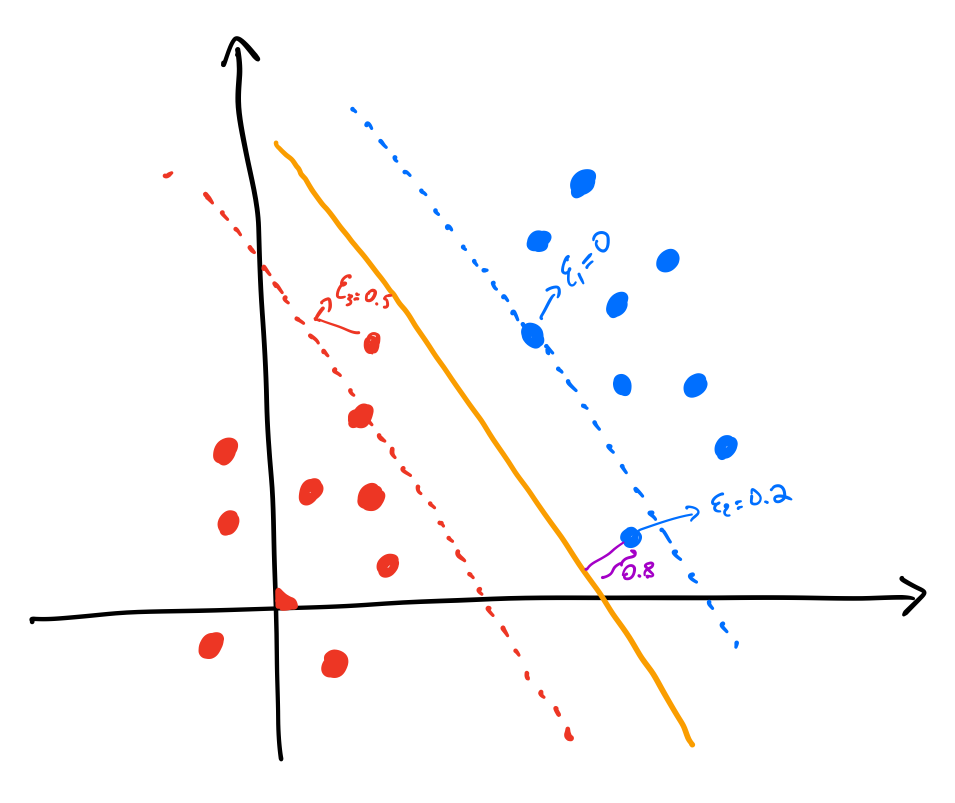
\includegraphics[scale=0.19]{./figs/SVM_Fig8.png}
\end{center}
}

\Sli{
A forma dual de nosso problema de otimização é muito similar ao que tínhamos apresentado na formulação das SVMs de margens rígidas (Equação 15), ou seja:

\begin{equation}\nonumber
	\boldsymbol{\alpha}^\ast = \argmax_{\boldsymbol{\alpha}}\left\{-\frac{1}{2}\sum_{i=1}^m\sum_{j=1}^m\alpha_i\alpha_jy_iy_j\boldsymbol{x}_i^T\boldsymbol{x}_j+\sum_{i=1}^m\alpha_i\right\}, 
\end{equation}
sujeito às seguintes restrições:

\begin{equation}\nonumber
	0 \leq \alpha_i \leq C,\ \ \forall i=1,2,\ldots,m
\end{equation}
e
\begin{equation}\nonumber
\sum_{i=1}^m\alpha_iy_i = 0.	
\end{equation}
}

\Sli{
\justify O nosso vetor de pesos $\boldsymbol{w}^\ast$ continua sendo calculado pela Equação 9. Já as variáveis de folga podem ser calculadas da seguinte maneira:

\begin{equation}
	\epsilon_i^\ast = \max\left\{0,1-\left[y_i\underbrace{\sum_{j=1}^my_j\alpha_j^\ast\boldsymbol{x}_j^T}_{\boldsymbol{w}^\ast}\boldsymbol{x}_i\right]+\theta^\ast\right\}.
\end{equation}

Notem que interessante: suponha uma amostra $\boldsymbol{x}_i$ que esteja sobre o hiperplano $H_1$, ou seja, $y_i = 1$. Neste caso, o termo $y_i\sum_{j=1}^my_j\alpha_j^\ast\boldsymbol{x}_j^T\boldsymbol{x}_i+\theta^\ast = (\boldsymbol{w}^\ast)^T\boldsymbol{x}_i +\theta^\ast= 1$. A Equação 21 acaba se transformando em $\epsilon_i^\ast = \max\{0,1-1\}= 0$, o que é verdade, pois $\boldsymbol{x}_i$ é um vetor de suporte.
}

\Sli{
Suponha, agora, uma outra amostra $\boldsymbol{x}_i$ que pertença à classe $1$, ou seja, $y_1=1$, mas está longe da margem. Neste caso, temos que:

\begin{equation}\nonumber
	y_i\sum_{j=1}^my_j\alpha_j^\ast\boldsymbol{x}_j^T\boldsymbol{x}_i+\theta^\ast = (\boldsymbol{w}^\ast)^T\boldsymbol{x}_i +\theta^\ast = k >> 1.
\end{equation}
A Equação 21 acaba se transformando em $\epsilon_i^\ast = \max\{0,1-k\}= 0$, o que é também verdade, pois $\boldsymbol{x}_i$ está longe da margem e, portanto, não precisa de variável da folga.\newline

Suponha, agora, que $\boldsymbol{x}_i$ pertença à classe $-1$, ou seja, $y_i=-1$, mas está longe da margem. Neste caso, temos que:

\begin{equation}\nonumber
y_i\sum_{j=1}^my_j\alpha_j^\ast\boldsymbol{x}_j^T\boldsymbol{x}_i+\theta^\ast = -(\boldsymbol{w}^\ast)^T\boldsymbol{x}_i -\theta^\ast = -k << -1. 
\end{equation}
}

\Sli{
Multiplicando-se a equação acima por $-1$, temos que:

\begin{equation}\nonumber
-(\boldsymbol{w}^\ast)^T\boldsymbol{x}_i -\theta^\ast = -k \implies (\boldsymbol{w}^\ast)^T\boldsymbol{x}_i +\theta^\ast = k >> 1.
\end{equation}

A Equação 21 acaba se transformando, novamente, em $\epsilon_i^\ast = \max\{0,1-k\}= 0$, o que é também verdade, pois $\boldsymbol{x}_i$ está longe da margem e, portanto, não precisa de variável de folga.

}

\Sli{
Agora, notem que temos duas condições de KKT:

\begin{equation}
	\alpha_i^\ast(y_i[(\boldsymbol{w}^\ast)^T\boldsymbol{x}_i+\theta]-1+\boldsymbol{\epsilon}^\ast) = 0,\ \forall i=1,2,\ldots,m.
\end{equation}
e
\begin{equation}
	(C-\alpha_i^\ast)\epsilon_i^\ast = 0.
\end{equation}

\justify No caso das SVMs com margens rígidas, tínhamos que os vetores de suporte eram as amostras $\boldsymbol{x}_i$ cujos multiplicadores de Lagrange $\alpha_i\geq0$. Agora, no caso das SVMs com margens suaves, temos que existem diferentes tipos de vetores de suporte de acordo com os valores de $\alpha_i$ e $\epsilon_i$.\newline

Caso $\alpha_i < C$, temos que $\epsilon_i^\ast = 0$ para a Equação 24 ser satisfeita. Ademais, pela Equação 23, concluímos que $\boldsymbol{x}_i$ é um vetor de suporte que está sobre a margem $H_1$ ou $H_2$ (depende de sua classe) ou está longe das margens. Este seria o mesmo caso das SVMs com margens rígidas.
}

\Sli{
Agora, caso $\alpha_i^\ast = C$, temos três possíveis situações:

\begin{enumerate}
	\item $\epsilon_i^\ast>1$: erros no conjunto de treinamento pois os vetores de suporte cruzam o hiperplano separador.
	\item $0\leq\epsilon_i^\ast<1$: amostras situadas entre as margens (não são erros, apenas estão violando as regras).
	\item $\epsilon_i^\ast = 0$: amostras sobre as margens ou longe delas.
\end{enumerate}
\vspace{-0.7cm}
\begin{center}
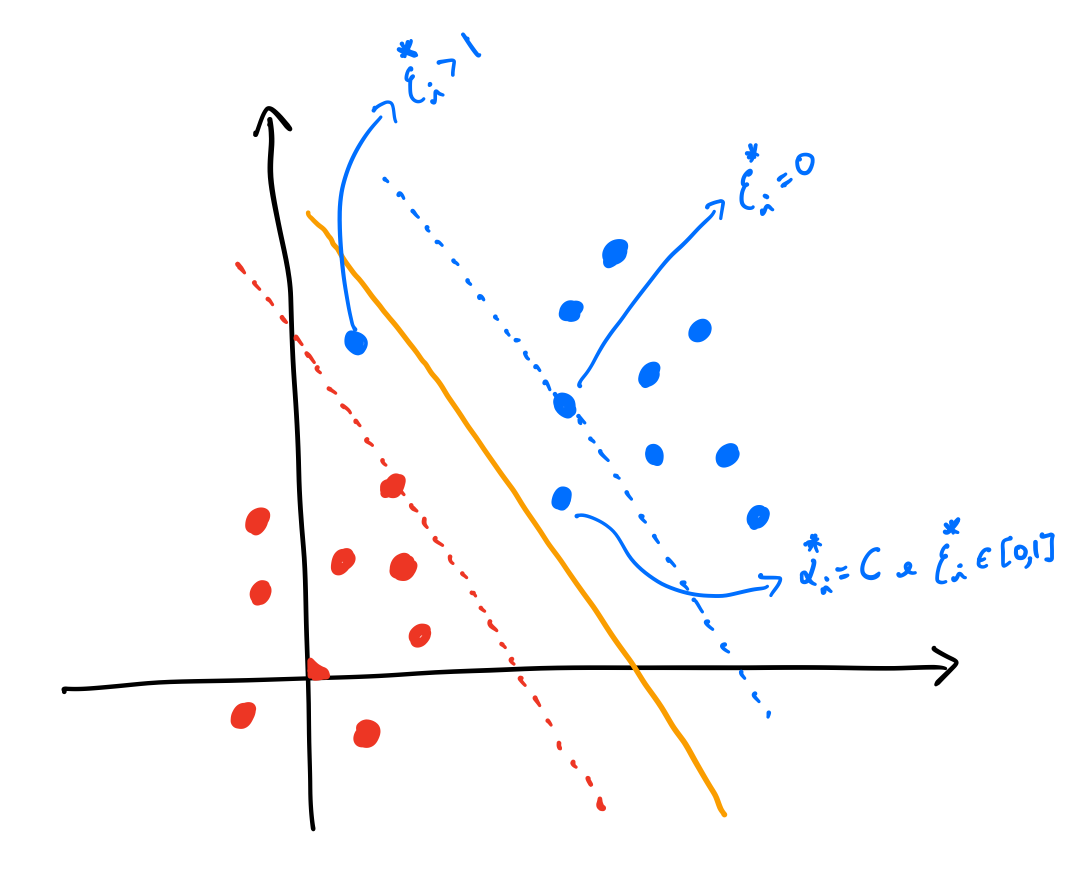
\includegraphics[scale=0.14]{./figs/SVM_Fig9.png}
\end{center}
}

\Sli{
Falta, agora, calcularmos $\theta^\ast$, que é computado pela média da Equação 18 sobre todos os vetores de suporte com $\alpha_i<C$, ou seja:

\begin{equation}
	\theta^\ast = \frac{1}{|{\cal V}|}\sum_{\boldsymbol{x}_i\in{\cal S}\wedge\alpha_i\ast<C}\left\{\frac{1}{y_i}-\sum_{\boldsymbol{x}_j\in{\cal S}}\alpha_j^\ast y_j\boldsymbol{x}_j^T\boldsymbol{x}_i\right\}.
\end{equation}
Lembrando que ${\cal S}$ denota o conjunto de todos os vetores de suporte (livres e limitados), e ${\cal V}$ denota os vetores de suporte limitados apenas, ou seja, aquelas amostras para as quais $\alpha_i^\ast<C$.
}

\SliT{SVMs Não-Lineares}{
\justify Quando temos dados que são linearmente separáveis, podemos fazer uso das SVMs com margens suaves ou rígidas, como vimos anteriormente. No entanto, como podemos lidar com o caso de dados não lineares, visto que os modelos baseados em SVM aprendidos até agora consegue aprender apenas superfícies de decisão lineares? \textbf{A solução é mapear os dados para um outro espaço de maior dimensão} Esta solução é também conhecida por \emph{kernel trick}.
\vspace{-.4cm} 
\begin{center}
\begin{tabular}{cc}
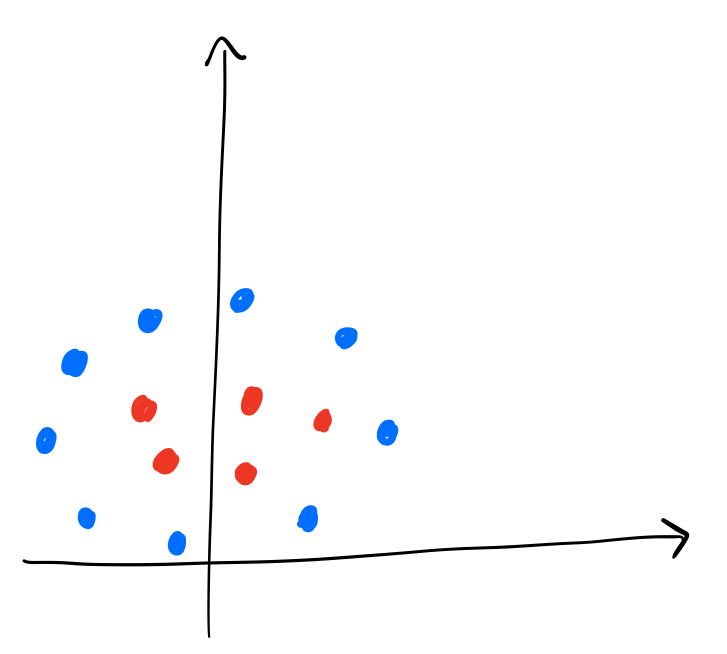
\includegraphics[scale=0.17]{./figs/SVM_Fig10.png} &\hspace{2cm} 
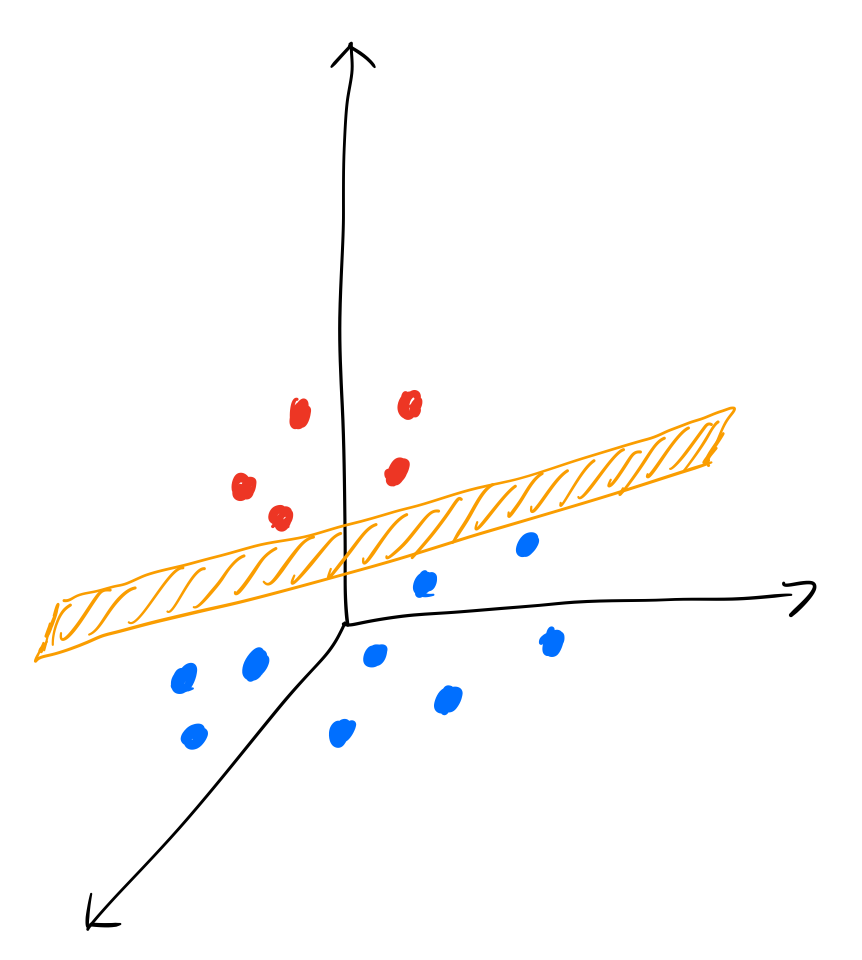
\includegraphics[scale=0.13]{./figs/SVM_Fig11.png}	
\end{tabular}
\end{center}
}

\Sli{
Como é a ideia dessa \textbf{função de mapeamento}? Suponha que tenhamos o seguinte exemplo:

\begin{itemize}
	\item $\phi:\mathbb{R}^2\rightarrow\mathbb{R}^3$ (função de mapeamento)
	\item $\boldsymbol{x}\in\mathbb{R}^2$ (elemento de entrada)
	\item $\phi(\boldsymbol{x}) = \phi(x^1,x^2) = ((x^1)^2,\sqrt{2}x^1x^2,(x^2)^2)$ (elemento mapeado)
\end{itemize}
\justify A ideia é que os dados estarão melhor distribuídos em espaços com maiores dimensões. O \textbf{Teorema de Cover} diz que um problema de classificação de padrões mapeado não-linearmente para um espaço de maior dimensão é mais provável de ser linearmente separável do que no espaço original, dado que o espaço não é densamente povoado.
}

\Sli{
Novamente, o problema dual é dado pela seguinte formulação:

\begin{equation}
	\boldsymbol{\alpha}^\ast = \argmax_{\boldsymbol{\alpha}}\left\{-\frac{1}{2}\sum_{i=1}^m\sum_{j=1}^m\alpha_i\alpha_jy_iy_j\phi(\boldsymbol{x}_i)\phi(\boldsymbol{x}_j)+\sum_{i=1}^m\alpha_i\right\}.
\end{equation}
A solução é dada, também, de maneira similar, ou seja:

\begin{equation}
h_{\boldsymbol{w}^\ast}(x) = \sign\{(\boldsymbol{w}^\ast)^T\boldsymbol{x}+\theta^\ast\} = \sign\left\{\underbrace{\sum_{\boldsymbol{x}_i\in{\cal S}}y_i\alpha^\ast_i\phi(\boldsymbol{x}_i)}_{\boldsymbol{w}^\ast}\phi(\boldsymbol{x})+\theta^\ast\right\}.
\end{equation}
}

\Sli{
O parâmetro $\theta^\ast$, calculado na Equação 24, também pode ser obtido de maneira similar:

\begin{equation}
	\theta^\ast = \frac{1}{|{\cal V}|}\sum_{\boldsymbol{x}_i\in{\cal S}\wedge\alpha_i\ast<C}\left\{\frac{1}{y_i}-\sum_{\boldsymbol{x}_j\in{\cal S}}\alpha_j^\ast y_j\phi(\boldsymbol{x}_j)\phi(\boldsymbol{x}_i)\right\}.
\end{equation}

\justify A pergunta é: como projetar o operador de mapeamento $\phi$? Uma solução é por meio das funções \emph{kernel}, em que não é necessário conhecer um mapeamento específico para determinado dado, apenas como realizar produtos escalares no novo espaço.
}

\Sli{
Uma função de kernel $K$ é definida, basicamente, como segue:

\begin{equation}
	K(\boldsymbol{x}_i,\boldsymbol{x}_j) = \phi(\boldsymbol{x}_i)^T\phi(\boldsymbol{x}_j),
\end{equation}
ou seja, a função kernel recebe dois vetores no espaço de entrada e retorna o valor do produto escalar das amostras no espaço de maior dimensão. Esse é o então chamado \emph{kernel trick}. Vejamos o exemplo abaixo:

\begin{itemize}
	\item $\phi:\mathbb{R}^2\rightarrow\mathbb{R}^3$, $\phi(\boldsymbol{x}) = \phi(x^1,x^2) = ((x^1)^2,\sqrt{2}x^1x^2,(x^2)^2)$
	\item $\boldsymbol{x}_i = (x^1_i,x^2_i)$ e $\boldsymbol{x}_j = (x^1_j,x^2_j)$
	\item $K(\boldsymbol{x}_i,\boldsymbol{x}_j) = \phi(\boldsymbol{x}_i)^T\phi(\boldsymbol{x}_j) = \overbrace{((x^1_i)^2,\sqrt{2}x^1_ix^2_i,(x^2_i)^2)^T((x^1_j)^2,\sqrt{2}x^1_jx^2_j,(x^2_j)^2)}^{\text{produto interno}}=(x_i^1)^2(x_j^1)^2+\sqrt{2}x^1_ix^2_i\sqrt{2}x^1_jx^2_j+(x^1_j)^2(x^2_j)^2 = ((x_i^1)^2(x_j^1)^2+2x^1_ix^2_ix^1_jx^2_j+(x_i^2)^2(x_j^2)^2$ 
\end{itemize}
}

\end{document}